\section{Planejamento de Projeto}

Para melhor entender as etapas de desenvolvimento, antes é preciso conhecer o contexto do problema que deu origem ao processo de idealização, definição de interface e fluxo de execução da ferramenta. \\

\textbf{Processo de idealização} \\

Atualmente, para que clientes façam o uso de estruturas de dados remotos, estes precisam encontrar um meio de buscá-los eventualmente antes de executar uma lógica que dependa dos dados. Isso sugere a escrita de um código encarregado de acessar serviços\footnote{
  Infraestrutura distribuída (servidores, banco de dados, etc) que responde à pedidos de operações oriundas de clientes em forma de requisições de API.
} em busca de dados pela rede.

No entanto, para que haja garantia na comunicação, ao buscar dados diretamente em pontos de acesso\footnote{
  Parte de uma interface exposta por um serviço através de um canal de comunicação.
} de uma API, cria-se um contrato de acesso entre o cliente e a interface do serviço. Isso porque, uma vez implementado o código de busca, é preciso uma garantia de que não haja mudanças que ponham em risco sua funcionalidade e, assim, comprometer parte da lógica da aplicação. Além de possíveis danos financeiros, perde-se tempo de desenvolvimento de reimplementação.

\begin{figure}[H]
  \centering
  \begin{tikzpicture}[font=\small]
    \node (client) at (-3,0) {
\includegraphics[width=1.0cm]{figuras/client}};
    \node[right of=client] (clientFetchCode) at (-2.2,0.7) {
\includegraphics[width=1.1cm]{figuras/code}};
    \node[below of=clientFetchCode, node distance=1.6cm] (clientLogicCode) {
\includegraphics[width=1.1cm]{figuras/code}};
    \node[rectangle,minimum width=0.8cm, minimum height=3cm,draw,right of=clientFetchCode, node distance=3.0cm] (api) {API};
    \node[right of=api, node distance=1.8cm] (server) {
\includegraphics[width=1.0cm]{figuras/server}};
    \node[below of=server, node distance=1.8cm] (datastore) {
\includegraphics[width=1.0cm]{figuras/database}};
    \node[above of=server, node distance=1.8cm] (json) {
\includegraphics[width=1.1cm]{figuras/code}};
    \node[cloud, cloud puffs=30, minimum width=11cm, minimum height=10cm, draw,style={scale=0.6}] (service) at (server) {};
    \node[below of=clientFetchCode,node distance=0.0cm] {\textless$busca$\textgreater};
    \node[below of=clientLogicCode,node distance=0.0cm] {\textless$logica$\textgreater};
    \node[below of=json,node distance=0.0cm] {\{data\}};
    \node[below of=service,node distance=3.6cm] {Serviço};
    \node[below of=client,node distance=1.8cm] {\ldots};
    \node[right of=server,node distance=1.8cm] {\ldots};
    \draw[decorate,decoration={brace,raise=0.2cm,mirror}] ([yshift=6pt]clientFetchCode.north west) -- ([yshift=-12pt]clientLogicCode.south west);
    \draw [->] ([yshift=0.25cm]clientFetchCode.east) -- ([yshift=0.25cm]api.west);
    \draw [->] (api) -- (clientFetchCode);
  \end{tikzpicture}
  \caption{Contrato entre cliente e serviço na busca de dados}
\end{figure}

Atualmente, um dos problemas mais comuns de quebra de contrato entre API's e clientes ocorre em serviços que implementam o estilo de arquitetura REST. Em REST, pequenas mudanças como a de fluxo de dados\footnote{
  Fluxo de acesso do cliente em pontos de acesso para a busca de uma representação da estrutura total do serviço.
} podem causar instabilidade e o versionamento desnecessário de sua interface. Já em arquiteturas como GraphQL, o risco para esse tipo de mudança é baixo, pois não limita na interface a forma que clientes façam o acesso em busca de dados.

Vale lembrar que existem mudanças de diferentes níveis de impacto e complexidade de resolução. Por exemplo, mudanças como a de fluxo de dados ou estilo de arquitetura são possíveis de serem evitadas, pois afetam apenas o código de busca. Já mudanças como a alteração de campos da estrutura de dados são mais difíceis de serem resolvidas, pois seu acoplamento vai além do código de busca, podendo estar presente na lógica da aplicação.

\begin{figure}[H]
  \centering
  \begin{tikzpicture}[font=\small]
    \draw (-2,0) -- (-2,-5) (2,0) -- (2,-5);
    \node at (-2,0.3) {Cliente};
    \node at (2,0.3) {API (Serviço)};
    \node[dashed] (virtualData) at (-4,-1){
\includegraphics[width=1.1cm]{figuras/code}};
    \node[below of=virtualData,node distance=0.0cm] {\{data\}};
    \node (data) at (-4,-4.5) {
\includegraphics[width=1.1cm]{figuras/code}};
    \node[below of=data,node distance=0.0cm] {\{data\}};
    \node[cloud, cloud puffs=16,draw,minimum height=1.2cm] (cloudData) at (4,-2.5) {
\includegraphics[width=1.1cm]{figuras/code}};
    \node[below of=cloudData,node distance=0.0cm] {\{data\}};
    \draw[->] (-2,-1) -- node[midway,above] {requisição} (2,-1.5);
    \draw[<-] (-2,-2.5) -- node[midway,above] {resposta} (2,-2);
    \draw[->] (-2,-3) -- node[midway,above] {requisição} (2,-3.5);
    \draw[<-] (-2,-4.5) -- node[midway,above] {resposta} (2,-4);
  \end{tikzpicture}
  \caption{Fluxo de dados}
\end{figure}


\begin{figure}[H]
  \centering
  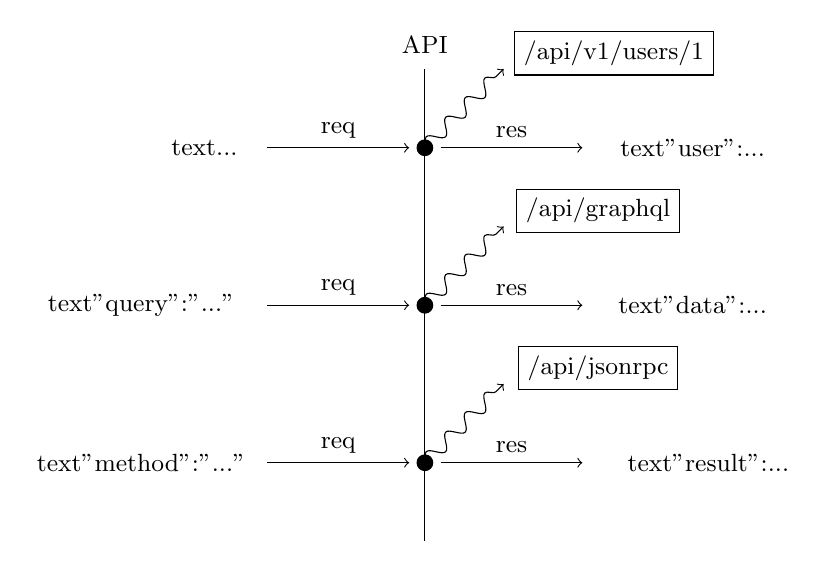
\begin{tikzpicture}[font=\small]
    \draw (0,1) -- (0,-5);
    \node at (0,1.3) {API};
    \node[draw,shape=circle,fill=black,style={scale=0.6}] at (0,0) {};
    \node[draw,shape=circle,fill=black,style={scale=0.6}] at (0,-2) {};
    \node[draw,shape=circle,fill=black,style={scale=0.6}] at (0,-4) {};
	\node at (-2.8,0) {\mintinline{text}{{...}}};
    \node at (-3.6,-2) {\mintinline{text}{{"query":"..."}}};
    \node at (-3.6,-4) {\mintinline{text}{{"method":"..."}}};
	\node at (3.4,0) {\mintinline{text}{{"user":{...}}}};
    \node at (3.4,-2) {\mintinline{text}{{"data":{...}}}};
    \node at (3.6,-4) {\mintinline{text}{{"result":{...}}}};
    \draw[->] (-2,0) -- node[midway,above] {req} (-0.2,0);
    \draw[->] (-2,-2) -- node[midway,above] {req} (-0.2,-2);
    \draw[->] (-2,-4) -- node[midway,above] {req} (-0.2,-4);
    \draw[->] (0.2,0) -- node[midway,above] {res} (2,0);
    \draw[->] (0.2,-2) -- node[midway,above] {res} (2,-2);
    \draw[->] (0.2,-4) -- node[midway,above] {res} (2,-4);
    \draw[->,decorate,decoration={snake,post length=1mm}] (0,0) -- (1,1);
    \draw[->,decorate,decoration={snake,post length=1mm}] (0,-2) -- (1,-1);
    \draw[->,decorate,decoration={snake,post length=1mm}] (0,-4) -- (1,-3);
    \node[draw] at (2.4,1.2) {/api/v1/users/1};
    \node[draw] at (2.2,-0.8) {/api/graphql};
    \node[draw] at (2.2,-2.8) {/api/jsonrpc};
  \end{tikzpicture}
  \caption{Requisição e resposta para estilos de arquitetura}
\end{figure}

A fim de melhorar a comunicação entre clientes e serviços através da possível prevenção de mudanças que levam a quebra de contrato, antes, fez-se necessário solucionar uma série de problemas descritos a seguir.

\begin{table}
  \begin{tabularx}{\linewidth}{>{\parskip1ex}X@{\kern4\tabcolsep}>{\parskip1ex}X}
    \toprule
    \hfil\bfseries Problema
    &
    \hfil\bfseries Solução
    \\\cmidrule(r{3\tabcolsep}){1-1}\cmidrule(l{-\tabcolsep}){2-2}

    (1) Dificuldade de realizar mudanças no fluxo de dados e estilo de arquitetura de uma API sem interferir no código de busca de clientes.\par
It's very nice\par
    (2) Não encontrado uma ferramenta para a resolução do problema anterior.\par
    (3) Criar uma linguagem para usar na comunicação entre código de busca e ferramenta para depois transformar em requisições de API.\par
    (4) Encontrar uma estrutura para se trabalhar com a sintaxe das consultas GraphQL descritas em texto.\par
    (5) Converter AST's em requisições para API's de serviços.\par
    (6) Escolher requisições de menor tempo de resposta para acesso de dados do cliente.
    
    &

    (1) Encontrar uma ferramenta para uso no cliente que evite o contrato de acesso nesses casos.\par
    (2) Construir uma ferramenta para clientes que faça a intermediação na comunicação entre seu código de busca e API do serviço.\par
    (3) Usar a linguagem GraphQL para expressar consulta de dados e depois analisar sintaxe a fim de transformar em requisições.\par
    (4) Converter a sintaxe das consultas em texto em estruturas AST para análise de dependências de dados.\par
    (5) Análise de metadados em pontos de acesso através de arquivos de descrição de API.\par
    (6) Algoritmo que analisa AST's e metadados de API's em busca o menor número de pontos de acesso e avalia o tamanho de resposta como critério.

    \\\bottomrule
  \end{tabularx}
  \caption{Problema e Solução}
\end{table}

Após solucionar os problemas, é proposto o primeiro protótipo do projeto onde prevê a criação de uma ferramenta que faça a intermediação na comunicação entre código de busca do cliente e API do serviço. Além disso, será necessário a reimplementação do código de busca para linguagem GraphQL, um arquivo para descrição da API disponibilizado pelo serviço e outro no cliente para configuração da ferramenta.

\begin{figure}[H]
  \centering
  \begin{tikzpicture}[font=\small]
    \node (client) at (-3,0) {
\includegraphics[width=1.0cm]{figuras/client}};
    \node[right of=client] (clientFetchCode) at (-2.2,0) {
\includegraphics[width=1.1cm]{figuras/code}};
    \node[below of=clientFetchCode, node distance=1.6cm] (clientLogicCode) {
\includegraphics[width=1.1cm]{figuras/code}};
    \node[above of=clientFetchCode, node distance=1.6cm] (clientConfigCode) {
\includegraphics[width=1.1cm]{figuras/code}};
    \node[circle,draw,right of=clientFetchCode,node distance=2.3cm] (schema) {Ferramenta};
    \node[rectangle,minimum width=0.8cm, minimum height=3cm,draw,node distance=1.8cm,right of=schema,node distance=2.7cm] (api) {API};
    \node[right of=api, node distance=1.8cm] (json) {
\includegraphics[width=1.1cm]{figuras/code}};
    \node[below of=json,node distance=1.8cm] (server) {
\includegraphics[width=1.0cm]{figuras/server}};
    \node[above of=json, node distance=1.8cm] (description) {
\includegraphics[width=1.1cm]{figuras/code}};
    \node[cloud, cloud puffs=30, minimum width=11cm, minimum height=10cm, draw,style={scale=0.6}] (service) at (json) {};
    \node[below of=clientFetchCode,node distance=0.0cm] {\textless$busca$\textgreater};
    \node[below of=clientLogicCode,node distance=0.0cm] {\textless$logica$\textgreater};
    \node[below of=clientConfigCode,node distance=0.0cm] {\textless$config$\textgreater};
    \node[below of=description,node distance=0.0cm] {\{desc\}};
    \node[below of=json,node distance=0.0cm] {\{data\}};
    \node[below of=service,node distance=3.6cm] {Serviço};
    \node[below of=client,node distance=1.8cm] {\ldots};
    \node[right of=json,node distance=1.8cm] {\ldots};
    \draw[decorate,decoration={brace,raise=0.2cm,mirror}] ([yshift=6pt]clientConfigCode.north west) -- ([yshift=-12pt]clientLogicCode.south west);
    \draw [->] ([yshift=0.25cm]clientFetchCode.east) -- ([yshift=0.25cm]schema.west);
    \draw [->] (schema) -- (clientFetchCode);
    \draw [->] ([yshift=0.25cm]schema.east) -- ([yshift=0.25cm]api.west);
    \draw [->] (api) -- (schema);
    \draw [->,dashed] (clientConfigCode) -| ([xshift=-0.25cm]schema.north);
    \draw [->,dashed] (description) -| ([xshift=0.25cm]schema.north);
  \end{tikzpicture}
  \caption{Proposta de modelo para evitar quebra de contrato}
\end{figure}

O novo modelo de comunicação procura, além de evitar a quebra de contrato, proporcionar um ambiente escalável para a composição de dados através de serviços baseados em JSON. Podendo ser aplicado em outras áreas de dificuldade como na adoção de novos estilos de arquiteturas e busca de dados em micro-serviços.

\begin{figure}[H]
  \centering
  \begin{tikzpicture}[font=\small]
    \node (client1) at (-2,0) {
\includegraphics[width=1.0cm]{figuras/client}};
    \node (client2) at (2,0) {
\includegraphics[width=1.0cm]{figuras/client}};
    \node[circle,draw,below of=client2,node distance=2.3cm] (schema) {Ferramenta};
    \node[cloud, cloud puffs=16, draw] (service1) at (-3,-6) {Serviço 1};
    \node[cloud, cloud puffs=16, draw] (service2) at (0,-6) {Serviço 2};
    \node[cloud, cloud puffs=16, draw] (service3) at (3,-6) {Serviço 3};
    \node[right of=service3,node distance=2.8cm] {\ldots};
    \draw [<->] (client1) -- (service1);
    \draw [<->] (client1) -- (service2);
    \draw [<->] (client1) -- (service3);
    \draw [<->] (client2) -- (schema);
    \draw [<->] (schema) -- (service1);
    \draw [<->] (schema) -- (service2);
    \draw [<->] (schema) -- (service3);
  \end{tikzpicture}
  \caption{Composição de serviços sem e com o modelo proposto}
\end{figure}

\textbf{Definição de interface} \\

Clientes que pensam em integrar a ferramenta em seu código esperam encontrar uma interface que apresente uma baixa curva de aprendizagem e que, acima de tudo, cause pouco impacto em sua base de código. Por isso, a ferramenta foi desenvolvida pensando em reutilizar ao máximo tecnologias promissoras ou já bem consolidadas no mercado de desenvolvimento.

A primeira ideia foi em utilizar GraphQL como linguagem para intermediação na comunicação. Além de promover a tecnologia, a ferramenta possibilita que o cliente escreva um código de busca que também funcione para interpretadores GraphQL. O outro caso é trabalhar com formatos abertos de descrição de API's, como por exemplo o JSON Hyper-Schema. Isso permite acelerar sua integração com serviços que já oferecem soluções de descrição de sua API's.

Para integrar a ferramenta em código de clientes, é preciso definir um arquivo de configuração contendo funções que descrevam informações de cada serviço a ser consultado. Após, gera-se um esquema GraphQL pela ferramenta a partir das funções de configuração de serviço. Por fim, é executado consultas no código de busca através do esquema gerado.

\begin{figure}[H]
  \centering
  \begin{minted}[frame=single,framesep=10pt,fontsize=\small]{text}
    import {adapter} from "graphql-jay-hyperschema"
  
    export function v1() {
      return fetch("/api/v1/schema").then((response) => {
        return response.json()
      }).then((schema) => {
        return {
          url: "/api/v1",
          schema,
          adapter,
          wrapper: {}
        }
      })
    }
  \end{minted}
  \caption{Exemplo de função de configuração para serviço REST}
\end{figure}

\begin{figure}[H]
  \centering
  \begin{minted}[frame=single,framesep=10pt,fontsize=\small]{text}
    import {graphql} from "graphql"
    import {composeSchema} from "graphql-jay"
    import services from "./services"
    
    composeSchema(...services).then((schema) => {
      graphql(schema, "{ user { id } }").then((response) => { 
        console.log(response.data)
      })
    })
  \end{minted}
  \caption{Exemplo de criação de esquema e execução de consulta}
\end{figure}

\textbf{Fluxo de execução} \\

Ao a efetuar a busca de dados entre clientes e serviços utilizando a ferramenta, dois fluxos de execução são realizados. O primeiro é o processo criação de esquema, que recebe como entrada funções de configuração de serviços e retorna um esquema GraphQL. O segundo é o processo de consulta de dados, onde a leva como entrada consultas em texto GraphQL e retorna estruturas de dados JSON remotas.

\begin{figure}[H]
  \centering
  \begin{tikzpicture}[font=\small,text width=5em, text centered]
    \node [rectangle,draw,minimum height=4em] (composeSchema) {Compor esquema unificado};
    \node [ellipse,draw,draw, above of=composeSchema,node distance=2cm] (services) {Serviços};
    \node [rectangle,draw,minimum height=4em, right of=composeSchema,node distance=3cm] (buildSchema) {Construir esquema para cada serviço};
    \node [rectangle,draw,minimum height=4em, right of=buildSchema,node distance=3cm] (wrapSchema) {Invólucrar campos de cada esquema};
    \node [rectangle,draw,minimum height=4em, right of=wrapSchema,node distance=3cm] (deepExtendSchema) {Unificar todos os esquemas};
    \node [ellipse,draw, above of=deepExtendSchema,node distance=2cm] (schema) {Esquema};
    \draw [->] (composeSchema) -- (buildSchema);
    \draw [->] (buildSchema) -- (wrapSchema);
    \draw [->] (wrapSchema) -- (deepExtendSchema);
    \draw [->,dashed] (services) -- (composeSchema);
    \draw [->,dashed] (deepExtendSchema) -- (schema);
  \end{tikzpicture}
  \caption{Criação de esquema}
\end{figure}

O processo de criação de esquema começa resolvendo cada função de configuração de serviço e construindo um esquema GraphQL para cada um. Após, por razões de preferência de desenvolvimento, é feito o invólucro dos campos de cada esquema e para cada um estende-se até gerar um esquema unificado.

\begin{figure}[H]
  \centering
  \begin{tikzpicture}[font=\small,text width=5em, text centered]
    \node [rectangle,draw,minimum height=4em] (simplifyAST) {Simplificar AST};
    \node [ellipse,draw, above of=simplifyAST,node distance=2cm] (services) {Consulta};
    \node [rectangle,draw,minimum height=4em, below of=simplifyAST,node distance=2cm] (transformAST) {Transformar AST para cada serviço};
    \node [rectangle,draw,minimum height=4em, right of=transformAST,node distance=3cm] (reduceASTs) {Reduzir AST de cada serviço};
    \node [rectangle,draw,minimum height=4em, right of=reduceASTs,node distance=3cm] (unwrapAST) {Desfazer invólucro de cada AST};
    \node [rectangle,draw,minimum height=4em, right of=unwrapAST,node distance=3cm] (fetchData) {Realizar busca dados para cada serviço};
    \node [rectangle,draw,minimum height=4em, above of=fetchData,node distance=2cm] (wrapData) {Invólucrar e unificar dados};
    \node [ellipse,draw, above of=wrapData,node distance=2cm] (schema) {Dados};
    \draw [->] (simplifyAST) -- (transformAST);
    \draw [->] (transformAST) -- (reduceASTs);
    \draw [->] (reduceASTs) -- (unwrapAST);
    \draw [->] (unwrapAST) -- (fetchData);
    \draw [->] (fetchData) -- (wrapData);
    \draw [->,dashed] (services) -- (simplifyAST);
    \draw [->,dashed] (wrapData) -- (schema);
  \end{tikzpicture}
  \caption{Consulta de dados}
\end{figure}

O processo de consulta de dados começa através de uma execução de consulta GraphQL. Primeiro é convertido a estrutura AST em um formato mais simplificado para se trabalhar. Após, transforma-se o AST principal em um AST especifico para cada serviço. Com as árvores de consulta, é feito a redução da árvore aplicando-se o algoritmo de busca. Após, é desfeito o invólucro de cada AST para poder realizar a busca de dados no serviço correspondente. Por fim, ao retornar os dados, realiza-se novamente o invólucro e estende-se cada dado até gerar um dado unificado.